  
\documentclass{beamer}
\usepackage{listings}
\usepackage{graphicx}
\usepackage{epstopdf}
\usepackage{hyperref}

\lstset{
		tabsize=4,
        basicstyle=\scriptsize,
        %upquote=true,
        aboveskip={1.5\baselineskip},
        columns=fixed,
        showstringspaces=false,
        extendedchars=true,
        breaklines=true,
        prebreak = \raisebox{0ex}[0ex][0ex]{\ensuremath{\hookleftarrow}},
		frame=tRBl,
		%frameround=tttf,
		numbers=left,
		numberstyle=\tiny,
		numbersep=5pt,
        showtabs=false,
        showspaces=false,
        showstringspaces=false,
        identifierstyle=\ttfamily,
        keywordstyle=\color[rgb]{0,0,1},
        commentstyle=\color[rgb]{0.133,0.545,0.133},
        stringstyle=\color[rgb]{0.627,0.126,0.941}
}

\usetheme{AnnArbor}
\usecolortheme{beaver}
\setbeamertemplate{note page}[plain]
\begin{document}

\title{Engineering Internet Applications}
\author[Konstantinos Karasavvas]{Konstantinos Karasavvas} %\\{\small Software Architect and Engineer}}

%http://www.linkedin.com/pub/konstantinos-karasavvas/14/64b/14b
\institute{CITY College}
\date{\today} 

\begin{frame}
  \titlepage
\end{frame}

\begin{frame}
\setcounter{tocdepth}{1}
\frametitle{Table of contents}
\tableofcontents
\end{frame} 





\section{Module Introduction} 
\begin{frame}\frametitle{Module Introduction} 
  \begin{itemize}
    \item Background 
    \begin{itemize}
      \item about me
      \item about you 
    \end{itemize}
    \pause
    \item Aims/Objectives
    \begin{itemize}
      \item Understand basic principles of Internet Applications
      \item Understand the architectural aspects
      \item Describe in detail web development (using Ruby and Sinatra)
      \item Understand the development process and organisation
    \end{itemize}
    \pause
    \item 3 hours per week
    \begin{itemize}
      \item 2 hours lectures
      \item 1 hour practical sessions (laptops/labs)
    \end{itemize}
    \pause
    \item Assessment
    \begin{itemize}
      \item Group project in Ruby/Sinatra (70\%)
      \item Quiz in Java (30\%)
    \end{itemize}
    
  \end{itemize}
\end{frame}



\begin{frame}\frametitle{Module Introduction, cont.} 
  \begin{itemize}
    \item Resources
    \begin{itemize}
      \item Why's (Poignant Guide) to Ruby
      \begin{itemize}
        \item http://mislav.uniqpath.com/poignant-guide/
      \end{itemize}
      \item Mr. Neighborly's Humble Little Ruby Book
      \begin{itemize}
        \item http://humblelittlerubybook.com/
      \end{itemize}
      \item Sinatra: Up and Running (http://it-ebooks.info/book/547/)
      \item https://www.ruby-lang.org/en/
      \item http://www.sinatrarb.com/
      \item http://sinatra-book.gittr.com/
      \item ...
    \end{itemize}
    \pause
    \item Contact
    \begin{itemize}
      \item \href{mailto:kkarasavvas@gmail.com}{kkarasavvas@gmail.com}
      \item Skype: kkarasavvas
      \item Twitter: kkarasavvas
      \item LinkedIn: \href{http://www.linkedin.com/pub/konstantinos-karasavvas/14/64b/14b}{Konstantinos Karasavvas}
    \end{itemize}
    \pause
    \item Ask, ask, and when in doubt ask!!!
    
  \end{itemize}
\end{frame}



\begin{frame}\frametitle{Expected Skills} 

  \begin{itemize}
  
    \item For the module
    \begin{itemize}
      \item Basic knowledge of desired OS
      \begin{itemize}
        \item Unix-based (recommended)
        \item Windows    \pause
      \end{itemize}

      \item Basic knowledge of HTML (CSS, JS)   \pause

      \item Basic understanding of database design  \pause
    
      \item Source Code Management tool (preferably Git)  \pause
    
      \item Quick to learn new tools and technologies  \pause
    
    \end{itemize}
    
    \item For the future
    \begin{itemize}
      \item Start a personal project   \pause
      \item Be passionate \pause (work hard!)
    \end{itemize}        
     
  \end{itemize}
\end{frame}



\begin{frame}\frametitle{Course Outline} 
  \begin{itemize}
    \item Week 1: Introduction to EIA and Ruby
    \item Week 2: Introduction to Ruby
    \item Week 3: Sinatra, MVC, ({\small ++}) and Tiny App demonstrating Web Dev.
    \item Week 4: Environments, Sessions, Error handling, ({\small ++}) 
    \item Week 5: Associations, Migrations, Web Authentication, Web Services
    \item Week 6: Consolidation Week
    \item Week 7: Client-side / Presentation 
    \item Week 8: Unit Testing, Functional Testing ({\small ++})
    \item Week 9: Web Development with Java
    \item Week 10: Web Development with Java 
    \item Week 11: Web Development with Java
    \item Week 12: Revision Week
  \end{itemize}
\end{frame}




\begin{frame}\frametitle{Coursework} 
  \begin{itemize}
    \item One project, in three phases / courseworks
    \begin{itemize}
      \item requirement analysis and design (group)
      \item basic implementation (group)
      \item advanced implementation  (individual)
    \end{itemize}   
    \pause
    \item Hard deadlines --- no delays!
    \item Feedback is essential for following phases
  \end{itemize}
\end{frame}




\section{World Wide Web} 
\begin{frame}[fragile]\frametitle{Basics (Technical)} 
% HTTP functions as a request-response protocol following the client-server model
  \begin{itemize}
    \item Hypertext Transfer Protocol (HTTP)
    \begin{itemize}
      \item request-response protocol
      \begin{itemize}
        \item application layer (TCP/IP \& OSI)
      \end{itemize}
      \item client-server model
      \item \texttt{GET}, \texttt{POST}, \texttt{DELETE}, ...
    \end{itemize}
  \end{itemize}
  
  \begin{lstlisting}[language=bash, escapechar={\#}]
$ telnet www.example.com 80  #\pause#
Trying 192.0.43.10...
Connected to www.example.com.
Escape character is '^]'.    #\pause#
GET / HTTP/1.1               #\pause#

HTTP/1.0 302 Found
Location: http://example.iana.org
Server: BigIP
Connection: Keep-Alive
Content-Length: 0
  \end{lstlisting}

\end{frame}




\begin{frame}\frametitle{Basics (Technical), cont.} 

  \begin{center}
    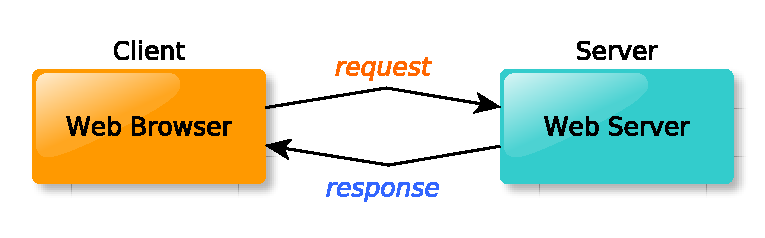
\includegraphics[scale=0.55]{diagrams/web_client_server.pdf}  
  \end{center}

  \pause
  
  \begin{itemize}
  
    \item Uniform Resource Identifier (\href{http://en.wikipedia.org/wiki/URI}{URI})
    \begin{itemize}
      \item URL, URN
    \end{itemize}
    
    \item \small \texttt{<scheme name>:<hierarchical path> [?<query>] [\#<fragment>] }

    \pause 
    
    \item Web Browser
    \begin{itemize}
      \item GET
      \item \texttt{http://example.com/path?param1=value1\&p2=v2}
    \end{itemize}
    

  \end{itemize}
\end{frame}





\begin{frame}\frametitle{Basics (Technical), cont.} 

  \begin{center}
    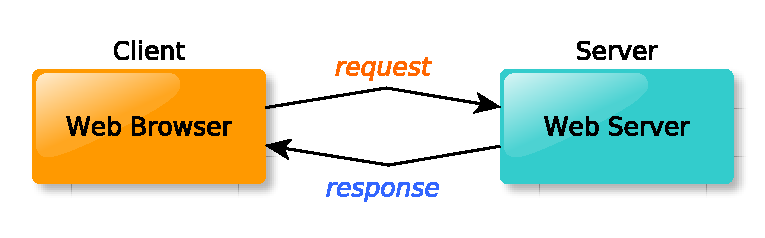
\includegraphics[scale=0.55]{diagrams/web_client_server.pdf}  
  \end{center}
  
  \begin{itemize}
  
    \item \texttt{response} body could contain anything
    \pause
    
    \item Web Browser is responsible for the presentation
    \begin{itemize}
      \item typically the browser renders HTML (data)
      \item CSS (layout)
      \item Javascript (client-side processing)
    \end{itemize}
    \pause
    
    \item We will primarily deal with the server side
    \pause
    
    \item More details later during architectural discussions

  \end{itemize}
\end{frame}






\section{Web Services} 
\begin{frame}\frametitle{Software Engineering: Abstraction \& Reuse} 
  \begin{itemize}

    \item Aims to simplify (for humans)  \pause

    \item Early assembly programming
    \begin{itemize}
      \item sequence of machine calls
    \end{itemize}
    \pause
    \item Procedural programming
    \begin{itemize}
      \item Structures (global)
      \item Procedures/functions
      \item Libraries
      \item C, Pascal, Basic, Modula, ...
    \end{itemize}
    \pause
    \item Object-oriented programming
    \begin{itemize}
      \item Encapsulation (inheritance/polymorphism)
      \item Interfaces
      \item Powerful class libraries
      \item Java, C++, C\#, Python, \textit{Ruby}, ...
    \end{itemize}
    
  \end{itemize}
\end{frame}



\begin{frame}\frametitle{Software Engineering: Abstraction \& Reuse, cont.} 
  \begin{itemize}

    \item Component\textit{-oriented programming}
    \begin{itemize}
      \item Defined rules and contracts for deployment and reuse
      \item Potentially distributed
      \item CORBA, COM/DCOM, EJB, CCA, ...
    \end{itemize}
    \pause
    \item Service\textit{-oriented programming}
    \begin{itemize}
      \item Service/contract-based abstractions
      \item Platform/OS independent, language independent
      \item Naturally distributed
      \item Autonomous (independence in 3rd party sense)
    \end{itemize}
    \pause
    \item Web Services
    \begin{itemize}
      \item Design focus is on service’s interface
      \item Loosely coupled (distributed) applications
      \begin{itemize}
        \item Integration at the interface (contract) level
        \item ...no implementation dependencies
      \end{itemize}

    \end{itemize}
    
  \end{itemize}
\end{frame}



\begin{frame}\frametitle{Web Services} 
  \begin{itemize}
    \item WWW originally designed for people to share information
    \begin{itemize}
      \item static content
    \end{itemize}    \pause
          
    \item Since early days: people have been using HTML forms as interfaces to access programs (CGI)
    \begin{itemize}
      \item dynamic content
    \end{itemize}    \pause
      
    \item More recently: machine to machine interaction      
    
    \pause
      
  \end{itemize}
  
\begin{quote}
``Web Service; just a Web page that is meant to be consumed by an autonomous program as opposed to a human.''
\end{quote}\par\raggedleft--- \textup{me :)}   
  
\end{frame}



\begin{frame}\frametitle{Web Services, cont.} 
  \begin{itemize}
  
    \item are application components
    \begin{itemize}
      \item basic
      \item part of very complex business and scientific processes
    \end{itemize}                \pause
          
    \item are distributed        \pause
    
    \item communicate using open protocols
    \begin{itemize}
      \item HTTP, SOAP, JSON, XML, ...
    \end{itemize}                \pause
      
    \item are platform neutral
    
    \pause
    
    \item can be implemented in different ways
    \begin{itemize}
      \item HTTP, REST or SOAP ?
    \end{itemize}  
    
  \end{itemize}
  
  \pause
  
  \begin{center}
    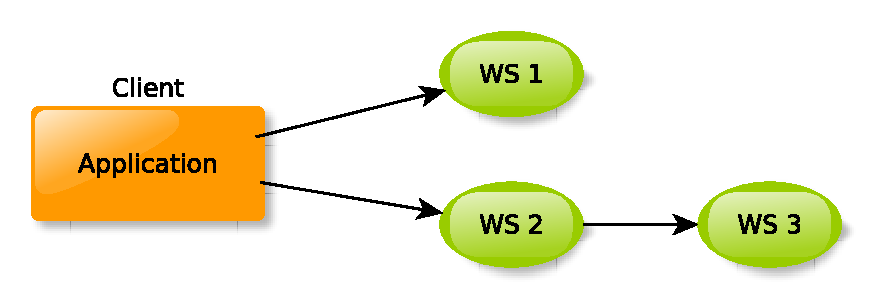
\includegraphics[scale=0.55]{diagrams/app_web_services.pdf}  
  \end{center}
  
\end{frame}




\section{Web Applications} 
\begin{frame}\frametitle{Web Applications} 
  \begin{itemize}
    
    \item Web site
    \begin{itemize}
      \item only static content?
      \item primarily informational (cnn.com) ?
    \end{itemize}                     \pause


    \item Web application
    \begin{itemize}
      \item allows user actions (gmail.com) ?
      \item allows login (personalisation, state, ...) ?
    \end{itemize}                                \pause

    \item Difference is lost nowadays
    
  \end{itemize}
\end{frame}




\begin{frame}\frametitle{Web Applications, cont.} 

  \begin{center}
    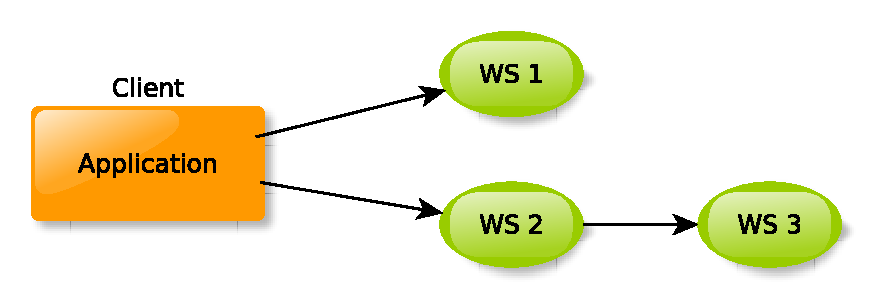
\includegraphics[scale=0.55]{diagrams/app_web_services.pdf}  
  \end{center}

  \pause
  
  \begin{center}
    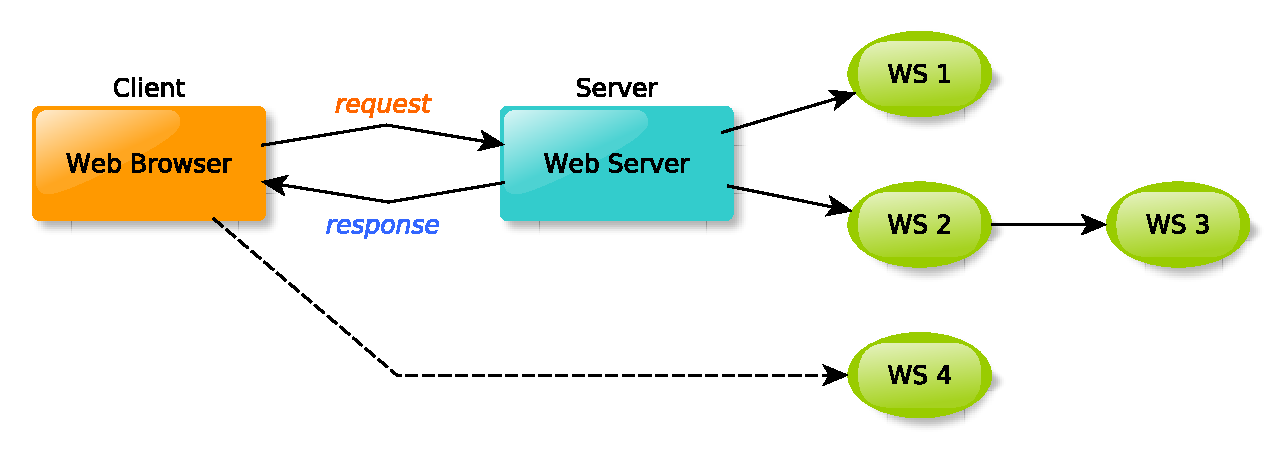
\includegraphics[scale=0.55]{diagrams/webapp_web_services.pdf}  
  \end{center}
  
\end{frame}



\begin{frame}\frametitle{Modern Web Application Characteristics} 
  \begin{itemize}

    \item Constant evolution \pause
    
    \item Huge target group  \pause
    
    \item High-quality UI    \pause
    
    \item Compressed development schedule  \pause
    
    \item Major impact of possible failure \pause
    
    \item Rapid technological changes  \pause
    
    \item Integration of heterogeneous technologies  \pause
    
    \item Need to support many platforms/browsers   \pause
    
    \item Security and privacy
    
  \end{itemize}
\end{frame}




\begin{frame}\frametitle{Web Application Frameworks (Ruby)} 
  \begin{itemize}

    \item Software frameworks
    \begin{itemize}
      \item Dynamic websites
      \item Web Applications
      \item Web Services
      \item Provide: security, database access, logging, sessions, ...
    \end{itemize}     
    \pause
    
    \item General Purpose frameworks 
    \begin{itemize}
      \item Sinatra
      \item Ruby on Rails
    \end{itemize}     
    \pause
    
    \item Wikis
    \begin{itemize}
      \item Instiki
    \end{itemize}     
    \pause

%    \item Content Management Systems
%    \begin{itemize}
%      \item Refinery CMS
%      \item Radiant
%    \end{itemize}     
    
    \item e-Commerce
    \begin{itemize}
      \item Spree
    \end{itemize}   
    
    \item ...

  \end{itemize}
\end{frame}


\begin{frame}\frametitle{Coursework} 
  \begin{itemize}
    \item Coursework 1
  \end{itemize}
\end{frame}


\end{document}
